\documentclass{beamer}
\usefonttheme[onlymath]{serif}
\usetheme{metropolis}

\usepackage[utf8]{inputenc}
\usepackage[sfdefault]{roboto}
\usepackage{graphicx}
\usepackage{amsmath}
\usepackage{amssymb}
\usepackage{multimedia}
\usepackage{graphicx}
\usepackage{minted}
\usepackage{transparent}
\usepackage{grid-system}
\usepackage{subfigure}

% ----------- MINTED DEFINE -----------
\definecolor{darkdarkgray}{rgb}{0.13,0.13,0.17}

\usemintedstyle{tomorrownight}
\newmintedfile[ccode]{cpp}{bgcolor=darkdarkgray, linenos}
% ----------- END MINTED DEFINE -----------

\newcommand{\norm}[1]{\left\| #1 \right\|}


\title{Image Stitching}
\author{Michael Stergianis}
\institute{University of Ontario Institute of Technology}
\date{\today}

\begin{document}
\frame{\titlepage}
\begin{frame}
  \frametitle{Why did I do image stitching?}
  I don't like user provided data to run programs, so I wanted to
  improve on assignment 2.
\end{frame}
\begin{frame}
  \frametitle{How does it work}
  \begin{itemize}
    \item It takes a list of two images at the command line
    \item Uses \texttt{opencv} functions to compute homography matrix
    \begin{itemize}
      \item Finds features using SIFT
      \item Matches features to find useful features using KNN matching
      \item Using correspondences computes homography matrix
    \end{itemize}
    \item Computes new canvas dimensions using transformation matrix
    \item Populates the new canvas
  \end{itemize}
\end{frame}
\begin{frame}
  \frametitle{What do the results look like?}
  \begin{figure}[ht]
    \centering
    \subfigure[Left]
    {\label{fig:img0} 
      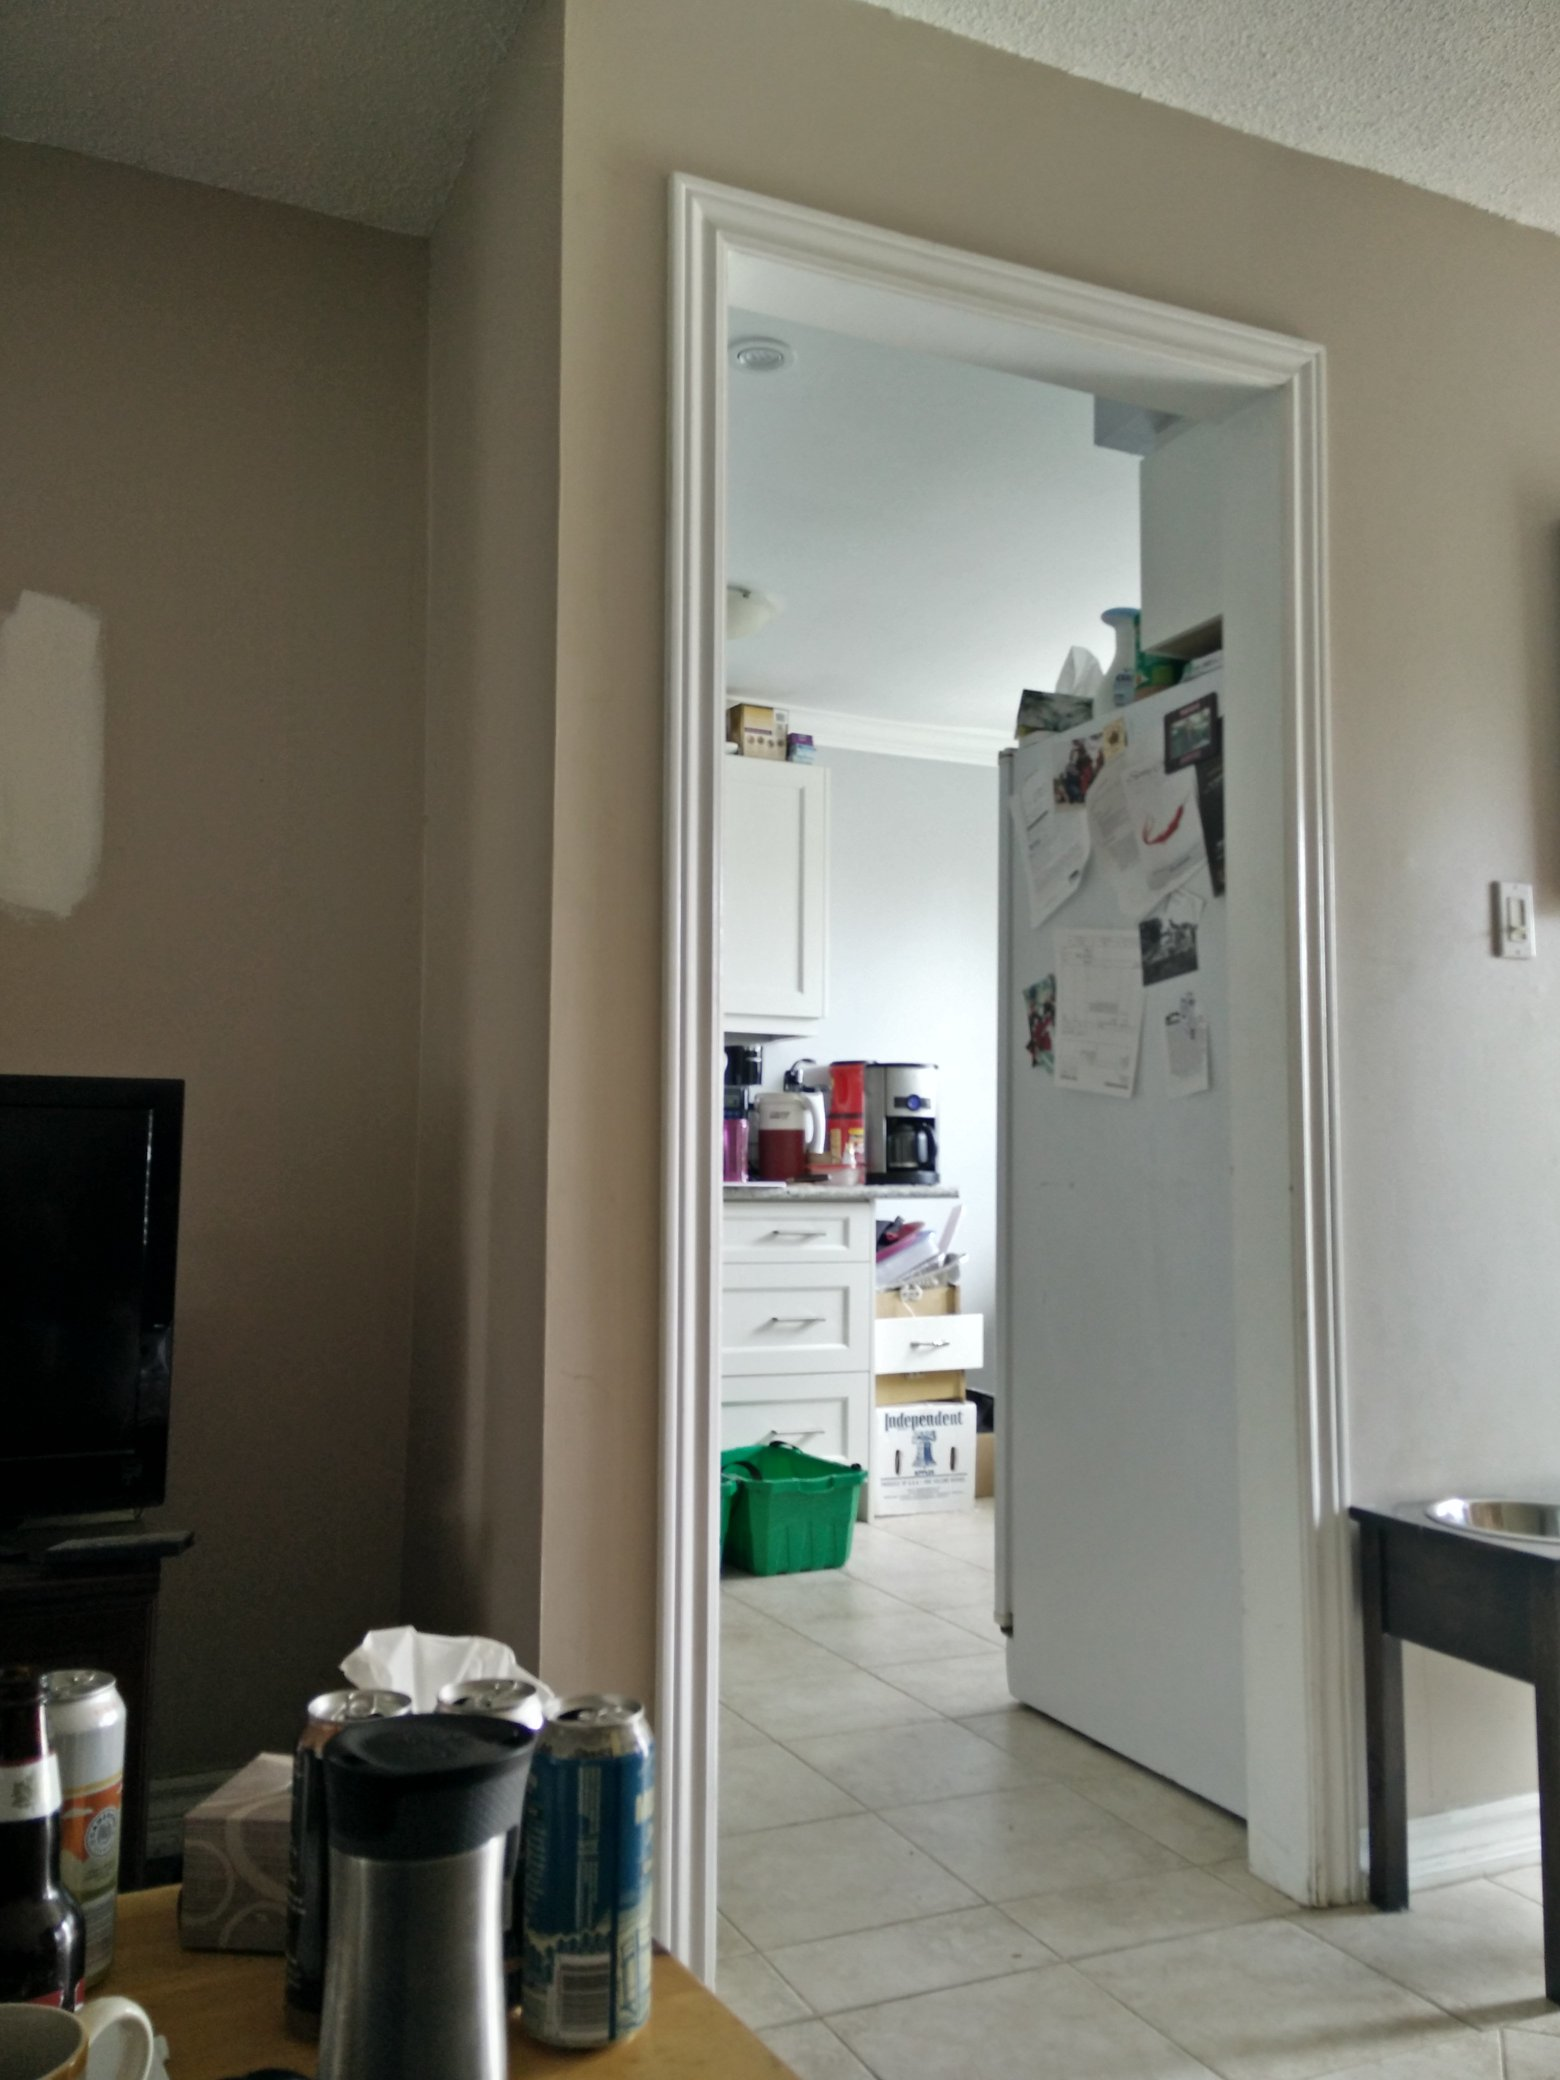
\includegraphics[width=.45\textwidth]{imgs/set_3/img0.jpg}}
    \subfigure[Right]
    {\label{fig:img1} 
      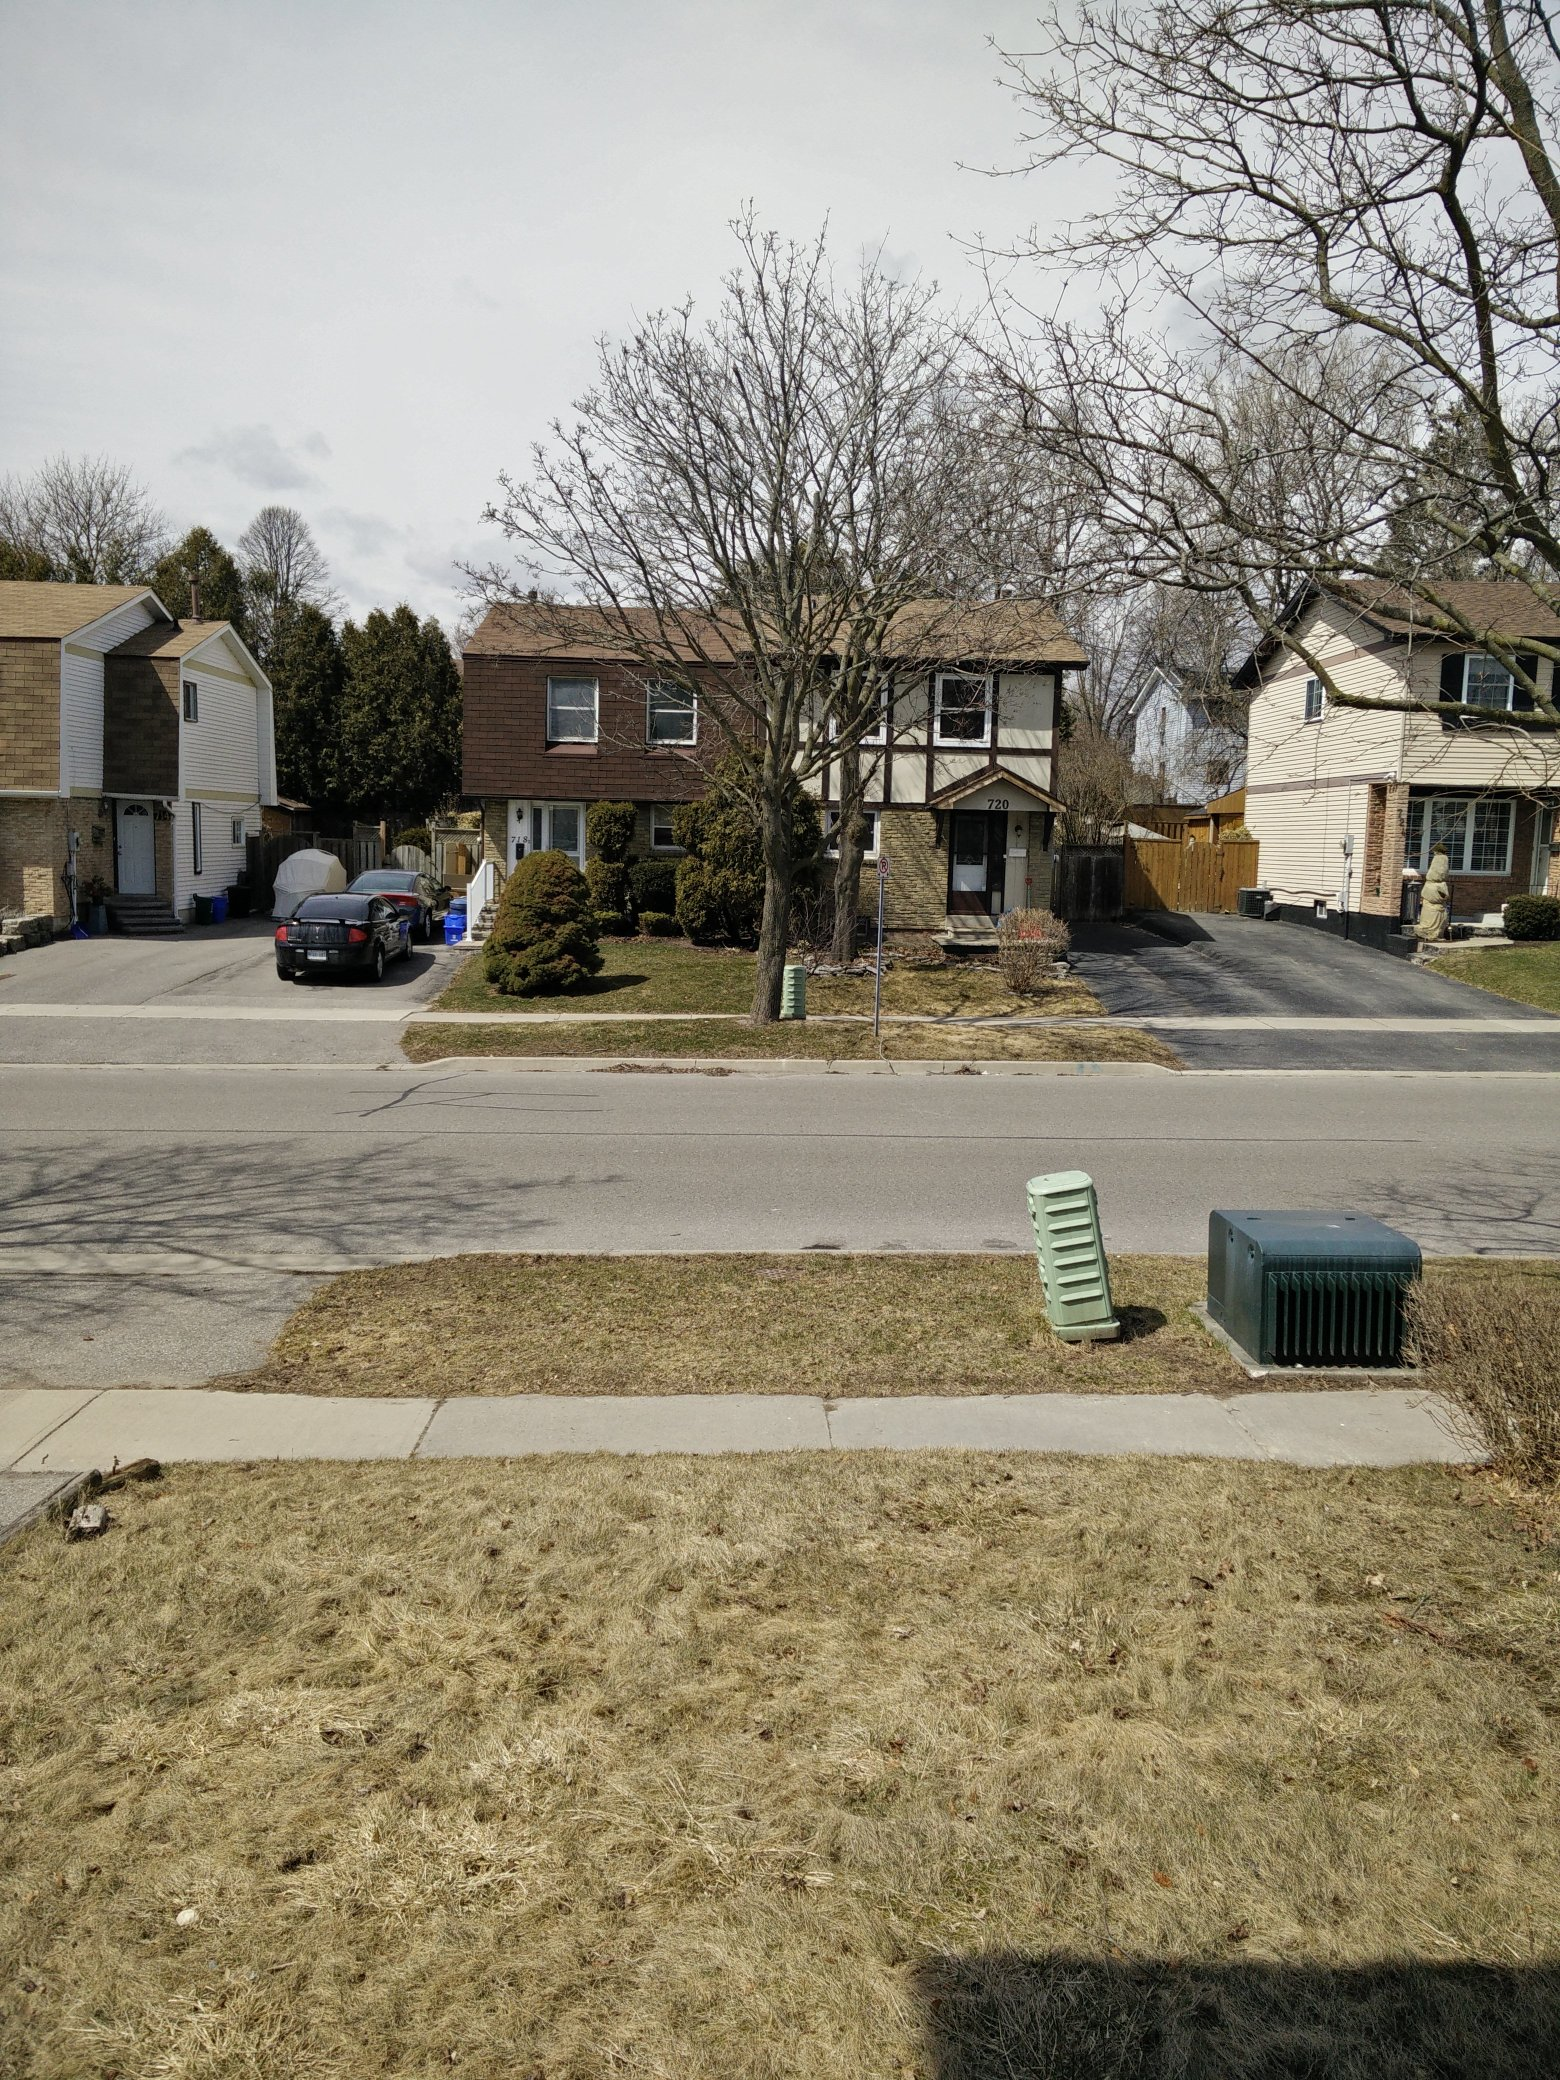
\includegraphics[width=.45\textwidth]{imgs/set_3/img1.jpg}}
    \caption{The original pair of images}
    \label{fig:pair}
  \end{figure}
\end{frame}
\begin{frame}
  \frametitle{What do the results look like?}
  \begin{figure}[ht]
    \centering
    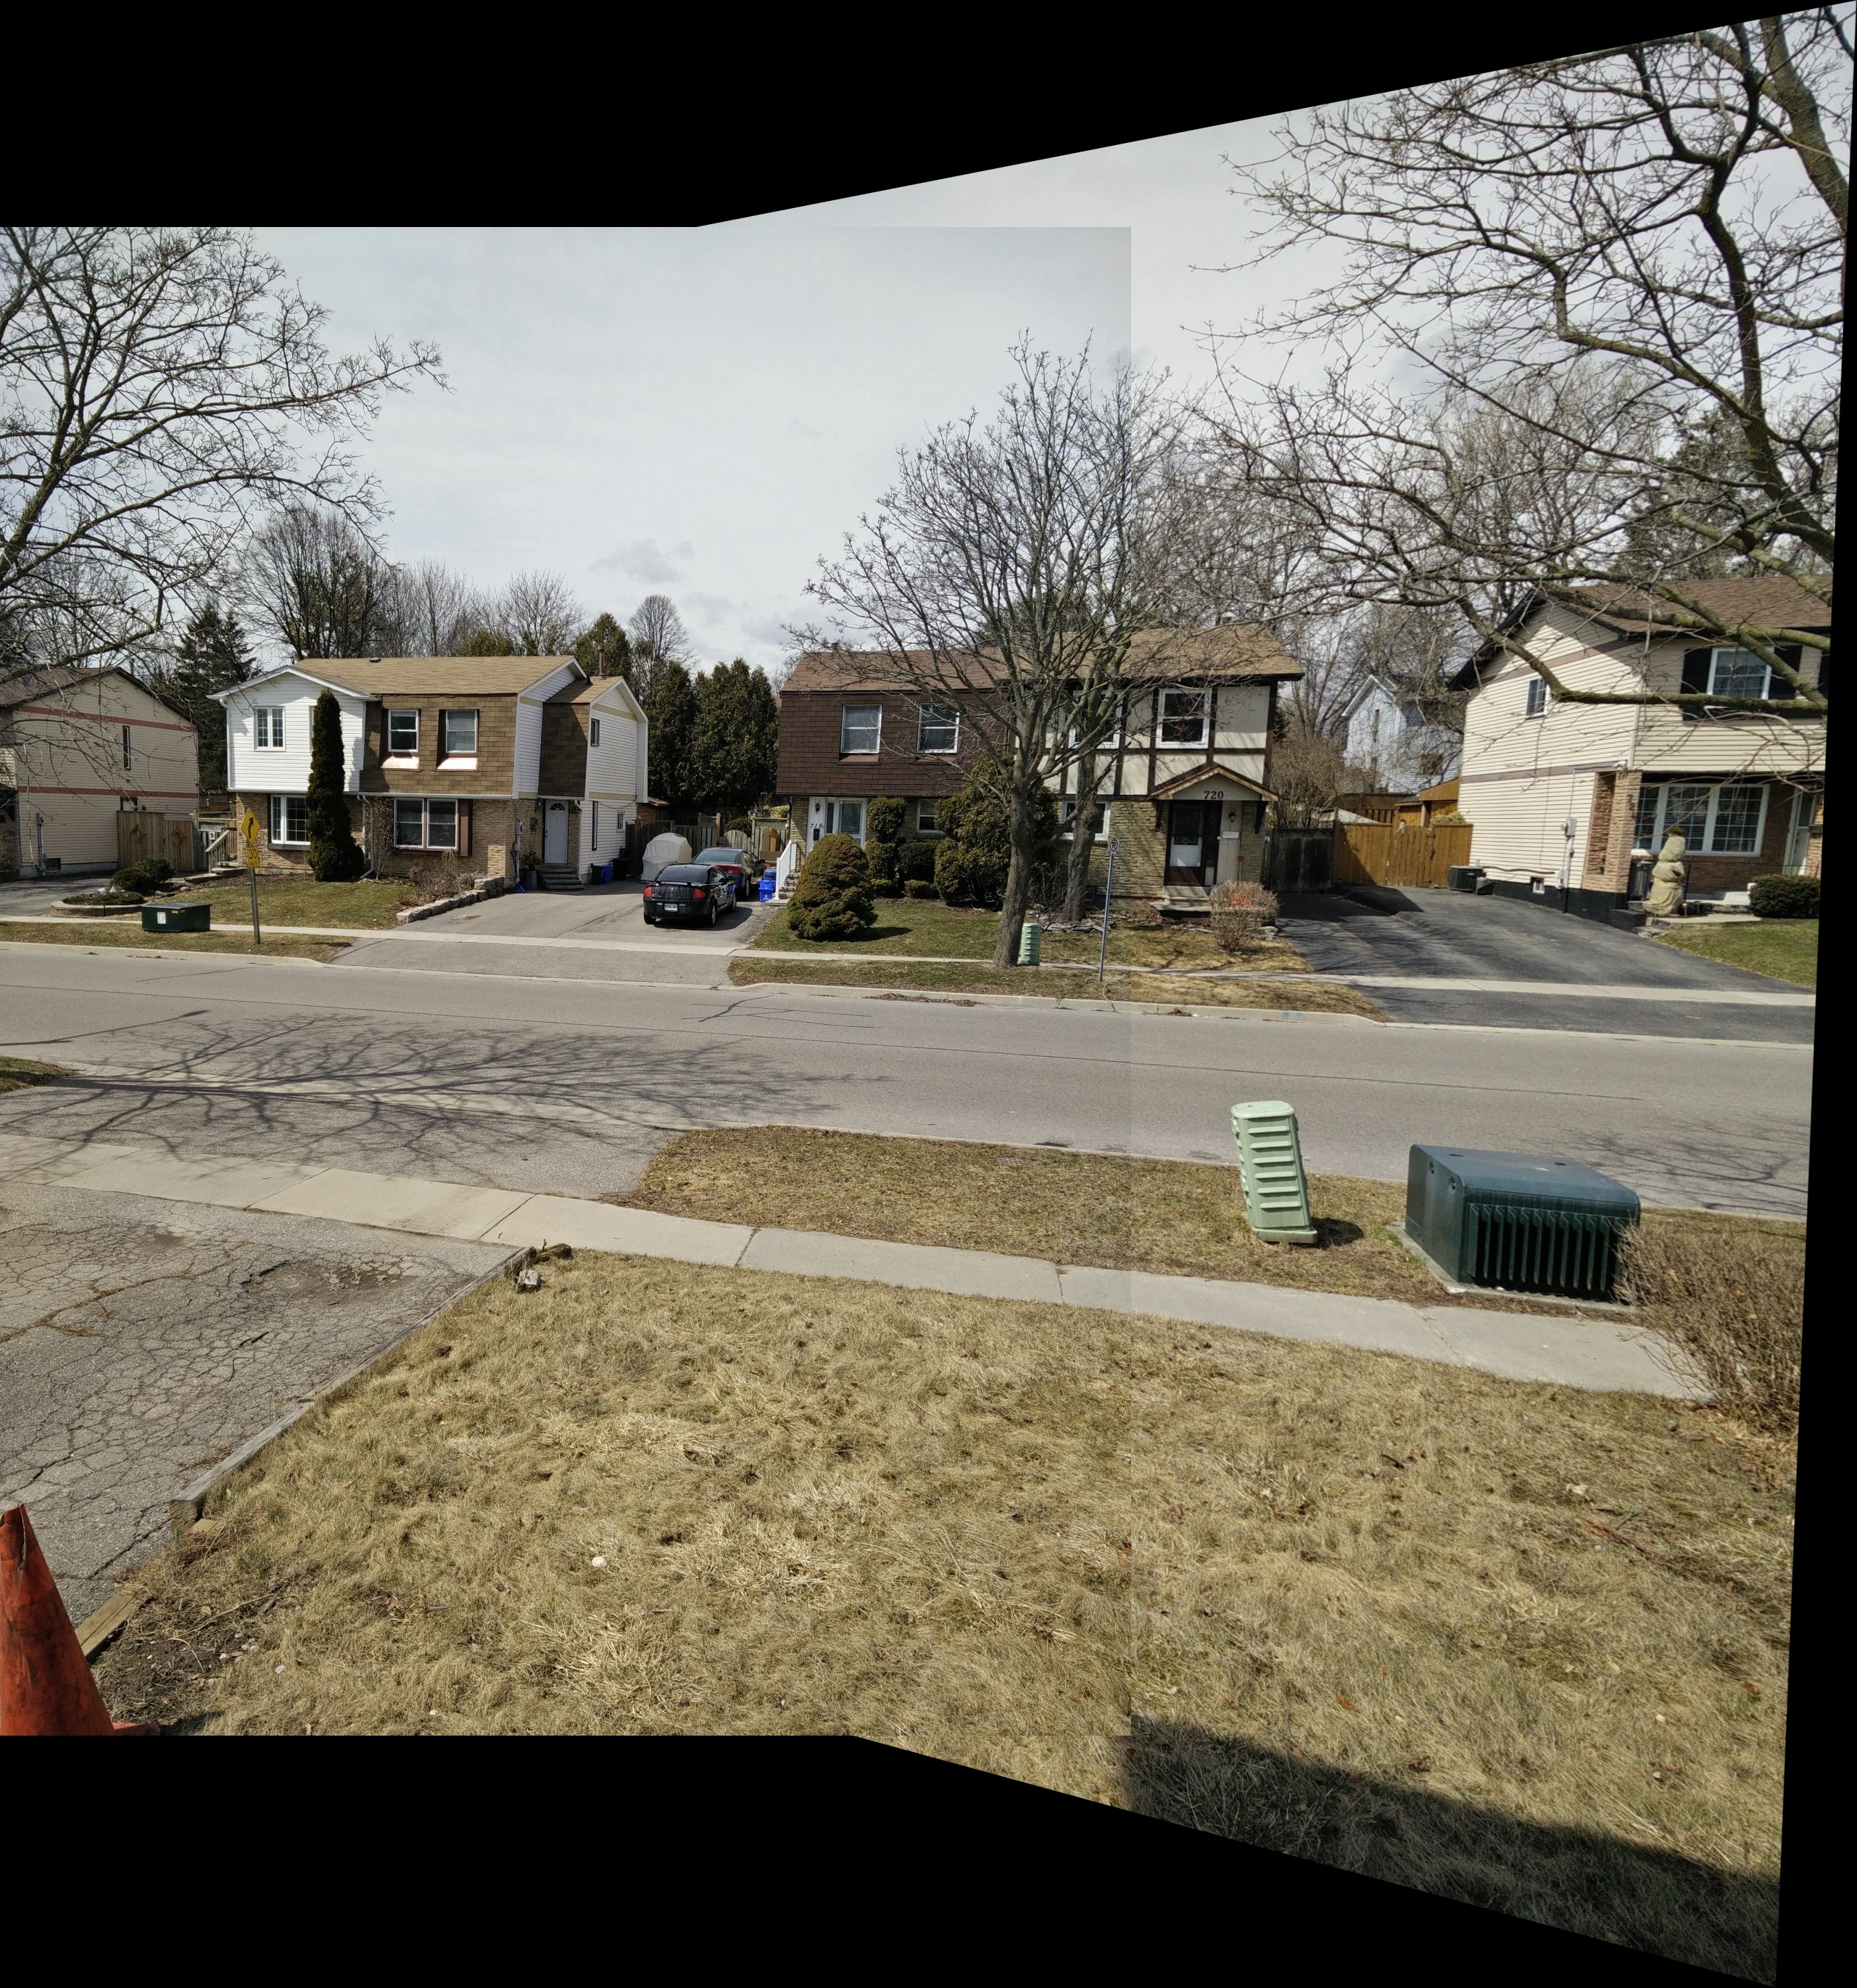
\includegraphics[width=.6\textwidth]{imgs/set_3/out.jpg}
    \caption{\label{fig:label} The stitched image}
  \end{figure}

\end{frame}
\end{document}
